\documentclass[12pt, a4paper]{article}
\usepackage[utf8]{inputenc}
\usepackage[T1]{fontenc}
\usepackage{amsmath, amssymb, amsthm}
\usepackage{geometry}
\usepackage{tikz}
\usepackage{pgfplots}
\pgfplotsset{compat=1.18}
\usepackage{float}
\usepackage{fancyhdr}

% Page Setup
\geometry{left=2.54cm, right=2.54cm, top=2.54cm, bottom=2.54cm}
\pagestyle{fancy}
\fancyhf{}
\lhead{Assignment 3}
\rhead{Mochiao Chen}
\cfoot{\thepage}

\title{\textbf{Assignment 3 Solutions}}
\author{Mochiao Chen \\ Student ID: 202442087}
\date{\today}

\begin{document}
\maketitle

\section*{Question 1}

\textbf{Problem Statement:} A monopolist faces the demand curve $Q = 150 - P$, and has a cost function $C(Q) = Q^2$.

\subsection*{(a) Profit-maximizing price and quantity}

First, we determine the inverse demand function and the marginal cost.
The demand is given by $Q = 150 - P$, which can be rewritten as:
$$ P = 150 - Q $$

The Total Revenue (TR) is:
$$ TR = P \cdot Q = (150 - Q)Q = 150Q - Q^2 $$

The Marginal Revenue (MR) is the derivative of TR with respect to Q:
$$ MR = \frac{dTR}{dQ} = 150 - 2Q $$

The Cost function is $C(Q) = Q^2$. The Marginal Cost (MC) is:
$$ MC = \frac{dC}{dQ} = 2Q $$

To maximize profit, the monopolist sets $MR = MC$:
$$ 150 - 2Q = 2Q $$
$$ 150 = 4Q $$
$$ Q^* = 37.5 $$

Substitute $Q^*$ back into the inverse demand function to find the price:
$$ P^* = 150 - 37.5 = 112.5 $$

\textbf{Result:} The profit-maximizing quantity is \textbf{37.5} and the price is \textbf{112.5}.

\subsection*{(b) Deadweight loss compared to the perfectly competitive outcome}

In a perfectly competitive market, Price equals Marginal Cost ($P = MC$).
$$ 150 - Q = 2Q $$
$$ 150 = 3Q $$
$$ Q_{PC} = 50 $$
$$ P_{PC} = 150 - 50 = 100 $$

The Deadweight Loss (DWL) is the area of the triangle formed by the demand curve, the marginal cost curve, and the quantities $Q^*$ and $Q_{PC}$.
The value of MC at the monopoly quantity ($Q=37.5$) is $MC = 2(37.5) = 75$.

$$ DWL = \frac{1}{2} \times (P^* - MC|_{Q^*}) \times (Q_{PC} - Q^*) $$
$$ DWL = \frac{1}{2} \times (112.5 - 75) \times (50 - 37.5) $$
$$ DWL = \frac{1}{2} \times 37.5 \times 12.5 $$
$$ DWL = 234.375 $$

\begin{center}
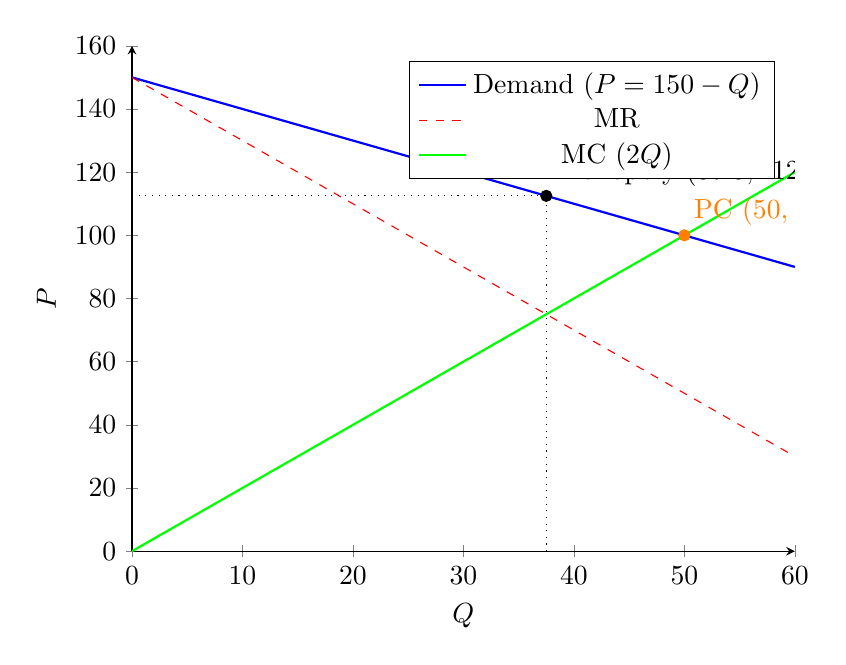
\begin{tikzpicture}
\begin{axis}[
    axis lines = left,
    xlabel = $Q$,
    ylabel = $P$,
    xmin=0, xmax=60,
    ymin=0, ymax=160,
    width=10cm, height=8cm,
    legend pos=north east
]
% Demand
\addplot [domain=0:60, color=blue, thick] {150 - x};
\addlegendentry{Demand ($P=150-Q$)}

% MR
\addplot [domain=0:60, color=red, dashed] {150 - 2*x};
\addlegendentry{MR}

% MC
\addplot [domain=0:60, color=green, thick] {2*x};
\addlegendentry{MC ($2Q$)}

% Monopoly Point
\addplot[mark=*, color=black] coordinates {(37.5, 112.5)} node[anchor=south west] {Monopoly ($37.5, 112.5$)};
\draw[dotted] (axis cs:37.5,0) -- (axis cs:37.5,112.5);
\draw[dotted] (axis cs:0,112.5) -- (axis cs:37.5,112.5);

% PC Point
\addplot[mark=*, color=orange] coordinates {(50, 100)} node[anchor=south west] {PC ($50, 100$)};

\end{axis}
\end{tikzpicture}
\end{center}

\subsection*{(c) Price ceiling at $P=60$}

The government imposes a price ceiling of $\bar{P} = 60$.
At $P=60$, the quantity demanded is:
$$ Q_d = 150 - 60 = 90 $$

The firm behaves as a price taker at $P=60$ as long as $P \ge MC$.
The firm's supply is determined where $P = MC$:
$$ 60 = 2Q $$
$$ Q_{supply} = 30 $$

Since the quantity supplied (30) is less than quantity demanded (90), the actual quantity traded is determined by supply.
$$ Q_{new} = 30 $$

The firm's profit is Total Revenue minus Total Cost:
$$ \pi = TR - TC = (P \cdot Q) - Q^2 $$
$$ \pi = (60 \cdot 30) - 30^2 $$
$$ \pi = 1800 - 900 = 900 $$

\textbf{Result:} The new quantity produced is \textbf{30}, and the firm's profit is \textbf{900}.

\newpage
\section*{Question 2}

\textbf{Problem Statement:} A monopoly faces an inverse demand curve, $p(y) = 100 - 2y$, and has constant marginal costs of 20.

\subsection*{(a) Profit-maximizing level of output}

The inverse demand function is $p(y) = 100 - 2y$.
The Total Revenue (TR) is:
$$ TR = p(y) \cdot y = (100 - 2y)y = 100y - 2y^2 $$

The Marginal Revenue (MR) is:
$$ MR = \frac{dTR}{dy} = 100 - 4y $$

The Marginal Cost (MC) is given as constant:
$$ MC = 20 $$

To maximize profit, set $MR = MC$:
$$ 100 - 4y = 20 $$
$$ 80 = 4y $$
$$ y^* = 20 $$

\textbf{Result:} The profit-maximizing level of output is \textbf{20}.

\subsection*{(b) Profit-maximizing price}

Substitute the profit-maximizing output ($y^* = 20$) into the inverse demand curve:
$$ p^* = 100 - 2(20) $$
$$ p^* = 100 - 40 = 60 $$

\textbf{Result:} The profit-maximizing price is \textbf{60}.

\subsection*{(c) Socially optimal price}

The socially optimal outcome occurs under perfect competition conditions where Price equals Marginal Cost ($P = MC$).
$$ p_{soc} = MC = 20 $$

\textbf{Result:} The socially optimal price is \textbf{20}.

\subsection*{(d) Socially optimal level of output}

Substitute the socially optimal price ($p_{soc} = 20$) into the inverse demand curve to find the quantity:
$$ 20 = 100 - 2y_{soc} $$
$$ 2y_{soc} = 80 $$
$$ y_{soc} = 40 $$

\textbf{Result:} The socially optimal level of output is \textbf{40}.

\subsection*{(e) Deadweight loss due to monopolistic behavior}

The Deadweight Loss (DWL) is the area of the triangle bounded by the demand curve, the marginal cost curve, and the quantities produced under monopoly ($y^*$) and social optimality ($y_{soc}$).

$$ DWL = \frac{1}{2} \times (p^* - MC) \times (y_{soc} - y^*) $$
$$ DWL = \frac{1}{2} \times (60 - 20) \times (40 - 20) $$
$$ DWL = \frac{1}{2} \times 40 \times 20 $$
$$ DWL = 400 $$

\begin{center}
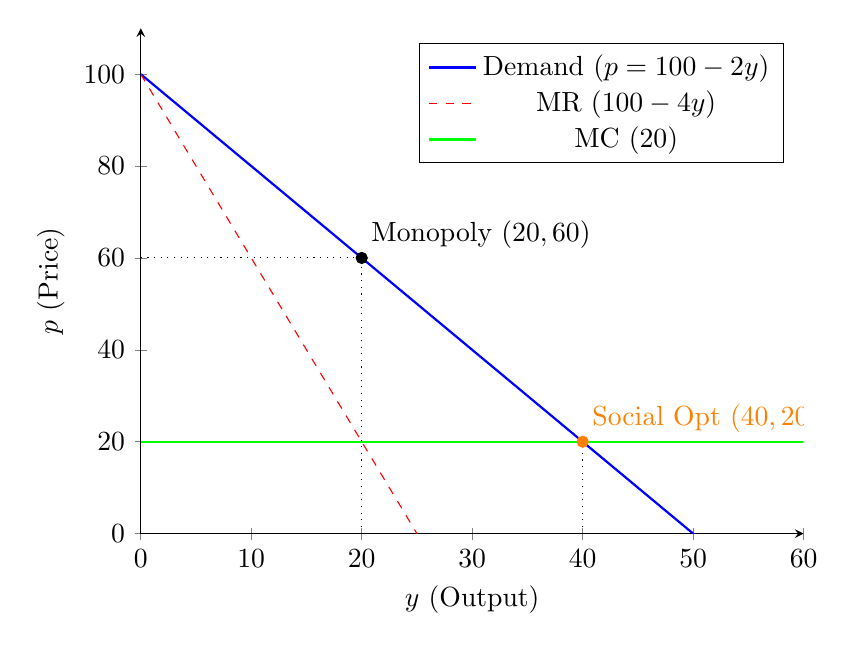
\begin{tikzpicture}
\begin{axis}[
    axis lines = left,
    xlabel = $y$ (Output),
    ylabel = $p$ (Price),
    xmin=0, xmax=60,
    ymin=0, ymax=110,
    width=10cm, height=8cm,
    legend pos=north east
]
% Demand
\addplot [domain=0:60, color=blue, thick] {100 - 2*x};
\addlegendentry{Demand ($p=100-2y$)}

% MR
\addplot [domain=0:30, color=red, dashed] {100 - 4*x};
\addlegendentry{MR ($100-4y$)}

% MC
\addplot [domain=0:60, color=green, thick] {20};
\addlegendentry{MC (20)}

% Monopoly Point
\addplot[mark=*, color=black] coordinates {(20, 60)} node[anchor=south west] {Monopoly ($20, 60$)};
\draw[dotted] (axis cs:20,0) -- (axis cs:20,60);
\draw[dotted] (axis cs:0,60) -- (axis cs:20,60);

% Social Optimum Point
\addplot[mark=*, color=orange] coordinates {(40, 20)} node[anchor=south west] {Social Opt ($40, 20$)};
\draw[dotted] (axis cs:40,0) -- (axis cs:40,20);

\end{axis}
\end{tikzpicture}
\end{center}

\textbf{Result:} The deadweight loss is \textbf{400}.

\subsection*{(f) Perfectly discriminating monopolist}

A perfectly discriminating monopolist (First-Degree Price Discrimination) charges each consumer their maximum willingness to pay.
In this scenario, the firm continues to sell as long as the price (willingness to pay) is greater than or equal to the marginal cost.
Therefore, the firm produces until $p(y) = MC$, which is the socially optimal quantity ($y = 40$).
Since the total surplus is maximized (though captured entirely by the producer) and the efficient quantity is produced, there is no efficiency loss.

\textbf{Result:} The deadweight loss in this case would be \textbf{0}.

\newpage
\section*{Question 3}

\textbf{Problem Statement:} A monopolist serves two separate markets with demand curves:
\begin{itemize}
    \item Market 1: $P_1 = 50 - Q_1$
    \item Market 2: $P_2 = 80 - 2Q_2$
\end{itemize}
The total cost function is $C(Q_1 + Q_2) = 10(Q_1 + Q_2)$, implying a constant Marginal Cost ($MC$) of 10.

\subsection*{(a) Price Discrimination: Prices and Quantities}

The monopolist maximizes profit by equating Marginal Revenue (MR) to Marginal Cost (MC) in each market separately.

\textbf{Market 1:}
$$ P_1 = 50 - Q_1 $$
$$ TR_1 = 50Q_1 - Q_1^2 $$
$$ MR_1 = 50 - 2Q_1 $$
Set $MR_1 = MC$:
$$ 50 - 2Q_1 = 10 \implies 2Q_1 = 40 \implies Q_1^* = 20 $$
Price: $P_1^* = 50 - 20 = 30$.

\textbf{Market 2:}
$$ P_2 = 80 - 2Q_2 $$
$$ TR_2 = 80Q_2 - 2Q_2^2 $$
$$ MR_2 = 80 - 4Q_2 $$
Set $MR_2 = MC$:
$$ 80 - 4Q_2 = 10 \implies 4Q_2 = 70 \implies Q_2^* = 17.5 $$
Price: $P_2^* = 80 - 2(17.5) = 45$.

\textbf{Result:}
\begin{itemize}
    \item Market 1: Price = \textbf{30}, Quantity = \textbf{20}.
    \item Market 2: Price = \textbf{45}, Quantity = \textbf{17.5}.
\end{itemize}

\subsection*{(b) Total Profit with Price Discrimination}

Profit is Total Revenue minus Total Cost. Since MC is constant, $\pi = (P_1 - MC)Q_1 + (P_2 - MC)Q_2$.
$$ \pi_{disc} = (30 - 10)20 + (45 - 10)17.5 $$
$$ \pi_{disc} = (20 \times 20) + (35 \times 17.5) $$
$$ \pi_{disc} = 400 + 612.5 = 1012.5 $$

\textbf{Result:} Total profit is \textbf{1012.5}.

\subsection*{(c) No Price Discrimination (Single Price)}

The monopolist must charge the same price $P$ in both markets. We first derive the aggregate demand curve by summing quantities horizontally.
$$ Q_1 = 50 - P \quad (\text{for } P \le 50) $$
$$ Q_2 = \frac{80 - P}{2} = 40 - 0.5P \quad (\text{for } P \le 80) $$
Total Quantity $Q = Q_1 + Q_2$:
$$ Q = (50 - P) + (40 - 0.5P) = 90 - 1.5P \quad (\text{valid for } P \le 50) $$
Inverse aggregate demand:
$$ 1.5P = 90 - Q \implies P = 60 - \frac{2}{3}Q $$

Total Revenue:
$$ TR = P \cdot Q = (60 - \frac{2}{3}Q)Q = 60Q - \frac{2}{3}Q^2 $$
Marginal Revenue:
$$ MR = 60 - \frac{4}{3}Q $$
Set $MR = MC$:
$$ 60 - \frac{4}{3}Q = 10 $$
$$ 50 = \frac{4}{3}Q \implies Q^* = 37.5 $$

Price:
$$ P^* = 60 - \frac{2}{3}(37.5) = 60 - 25 = 35 $$
(Note: $P=35 < 50$, so the assumption that both markets participate holds).

\textbf{Result:} The uniform price is \textbf{35}, and the total quantity sold is \textbf{37.5}.

\subsection*{(d) Comparison of Profits and Welfare}

\textbf{1. Price Discrimination Case:}
\begin{itemize}
    \item Producer Surplus ($PS$) = Profit = \textbf{1012.5}
    \item Consumer Surplus ($CS_1$) = $\frac{1}{2}(50 - 30)20 = 200$
    \item Consumer Surplus ($CS_2$) = $\frac{1}{2}(80 - 45)17.5 = 306.25$
    \item Total Welfare ($W_{disc}$) = $1012.5 + 200 + 306.25 = \textbf{1518.75}$
\end{itemize}

\textbf{2. Single Price Case ($P=35$):}
\begin{itemize}
    \item Quantities sold: $Q_1 = 50 - 35 = 15$; $Q_2 = 40 - 0.5(35) = 22.5$.
    \item Producer Surplus ($PS$) = $(35 - 10) \times 37.5 = \textbf{937.5}$
    \item Consumer Surplus ($CS_1$) = $\frac{1}{2}(50 - 35)15 = 112.5$
    \item Consumer Surplus ($CS_2$) = $\frac{1}{2}(80 - 35)22.5 = 506.25$
    \item Total Welfare ($W_{single}$) = $937.5 + 112.5 + 506.25 = \textbf{1556.25}$
\end{itemize}

\textbf{Conclusion:}
\begin{itemize}
    \item \textbf{Profit:} Higher with price discrimination ($1012.5 > 937.5$).
    \item \textbf{Total Welfare:} Higher without price discrimination ($1556.25 > 1518.75$).
\end{itemize}

\newpage
\section*{Question 4}

\textbf{Problem Statement:}
Demand: $D(p) = 1000 - p \implies P = 1000 - Q$.
Vertical structure: Perry Air (Upstream, Producer, $MC=0$) sells to Bubble Up (Downstream, Distributor) at price $c$. Bubble Up sells to consumers at price $P$.

\subsection*{(a) \& (b) Bubble Up's Equilibrium (Downstream)}

We solve this using backward induction. First, we analyze the distributor Bubble Up's behavior given a wholesale price $c$.
Bubble Up's Marginal Cost is the wholesale price $c$.
Bubble Up's Revenue:
$$ TR_{BU} = P \cdot Q = (1000 - Q)Q = 1000Q - Q^2 $$
$$ MR_{BU} = 1000 - 2Q $$
Set $MR_{BU} = MC_{BU}$:
$$ 1000 - 2Q = c $$
Solving for $Q$ gives Bubble Up's reaction function (derived demand for Perry Air):
$$ 2Q = 1000 - c \implies Q = 500 - 0.5c $$
However, we first need the value of $c$ determined by Perry Air (see next step).
Substituting $c=500$ (calculated in part c/d below):
$$ Q_{BU}^* = 500 - 0.5(500) = 250 $$
$$ P_{BU}^* = 1000 - 250 = 750 $$

\textbf{Result:}
\begin{itemize}
    \item (a) Equilibrium price charged by Bubble Up: \textbf{750}.
    \item (b) Equilibrium quantity sold by Bubble Up: \textbf{250}.
\end{itemize}

\subsection*{(c) \& (d) Perry Air's Equilibrium (Upstream)}

Perry Air behaves as a monopolist facing the derived demand from Bubble Up: $Q = 500 - 0.5c$.
Inverse derived demand: $0.5c = 500 - Q \implies c = 1000 - 2Q$.
Perry Air's Revenue (where price is $c$):
$$ TR_{PA} = c \cdot Q = (1000 - 2Q)Q = 1000Q - 2Q^2 $$
$$ MR_{PA} = 1000 - 4Q $$
Perry Air's Marginal Cost is 0.
Set $MR_{PA} = MC_{PA}$:
$$ 1000 - 4Q = 0 \implies 4Q = 1000 \implies Q_{PA}^* = 250 $$
Substitute $Q$ back to find the wholesale price $c$:
$$ c^* = 1000 - 2(250) = 500 $$

\textbf{Result:}
\begin{itemize}
    \item (c) Equilibrium price charged by Perry Air ($c$): \textbf{500}.
    \item (d) Equilibrium quantity sold by Perry Air: \textbf{250}.
\end{itemize}

\subsection*{(e) \& (f) Profits}

\textbf{Bubble Up Profit:}
$$ \pi_{BU} = (P - c)Q = (750 - 500) \times 250 = 250 \times 250 = 62,500 $$

\textbf{Perry Air Profit:}
$$ \pi_{PA} = (c - MC_{PA})Q = (500 - 0) \times 250 = 125,000 $$

\textbf{Result:}
\begin{itemize}
    \item (e) Bubble Up's profits: \textbf{62,500}.
    \item (f) Perry Air's profits: \textbf{125,000}.
\end{itemize}

\subsection*{(g) Consumer Surplus}

Consumer surplus is the area below the demand curve and above the price $P=750$.
$$ CS = \frac{1}{2} \times (P_{intercept} - P^*) \times Q^* $$
$$ CS = \frac{1}{2} \times (1000 - 750) \times 250 $$
$$ CS = \frac{1}{2} \times 250 \times 250 = 31,250 $$

\textbf{Result:} Consumer surplus is \textbf{31,250}.

\subsection*{(h) Buyout Price}

Perry Air needs to compensate Bubble Up for the loss of future profit stream.
Annual profit $\pi_{BU} = 62,500$. Interest rate $r = 0.1$.
Using the perpetuity formula:
$$ PV = \frac{\pi_{BU}}{r} = \frac{62,500}{0.1} = 625,000 $$

\textbf{Result:} The minimum lump sum payment is \textbf{625,000}.

\subsection*{(i) Merged Firm Equilibrium}

The merged firm eliminates the "double marginalization" problem. It faces the market demand directly with the true marginal cost ($MC=0$).
Demand: $P = 1000 - Q$.
$$ TR = 1000Q - Q^2 $$
$$ MR = 1000 - 2Q $$
Set $MR = MC$:
$$ 1000 - 2Q = 0 \implies Q_{merged} = 500 $$
$$ P_{merged} = 1000 - 500 = 500 $$

\textbf{Result:} New Price is \textbf{500}, New Quantity is \textbf{500}.

\subsection*{(j) Merged Firm Profits}

$$ \pi_{merged} = (P - MC)Q = (500 - 0) \times 500 = 250,000 $$
(Note: This is higher than the sum of separate profits $125,000 + 62,500 = 187,500$).

\textbf{Result:} The profits of the new merged firm are \textbf{250,000}.

\subsection*{(k) New Consumer Surplus and Comparison}

$$ CS_{new} = \frac{1}{2} \times (1000 - 500) \times 500 $$
$$ CS_{new} = \frac{1}{2} \times 500 \times 500 = 125,000 $$

\textbf{Comparison:}
Previous CS was 31,250. New CS is 125,000.
$$ \Delta CS = 125,000 - 31,250 = 93,750 $$

\textbf{Result:} The new consumer surplus is \textbf{125,000}. It is significantly higher (4 times higher) than the previous level because the elimination of double marginalization led to a lower price and higher output.

\newpage
\section*{Question 5}

\textbf{Problem Statement:}
\begin{itemize}
    \item Supply of small firms (Competitive Fringe): $S(p) = 100 + p$
    \item Market Demand: $D(p) = 200 - p$
    \item Large Firm Cost: $c(y) = 25y \implies MC_L = 25$
\end{itemize}

\subsection*{(a) Large firm output is zero (Competitive Equilibrium)}

If the large firm produces zero, the market price is determined by the intersection of the market demand and the supply of the small firms.
$$ S(p) = D(p) $$
$$ 100 + p = 200 - p $$
$$ 2p = 100 \implies p^* = 50 $$

Equilibrium Quantity ($Q$):
$$ Q = 200 - 50 = 150 $$

\textbf{Result:} Equilibrium price is \textbf{50}, Equilibrium quantity is \textbf{150}.

\subsection*{(b) Dominant Firm Model (Residual Demand)}

The large firm acts as a price leader facing the residual demand curve.
Residual Demand ($D_r$) = Market Demand ($D$) - Fringe Supply ($S$).
$$ y = D(p) - S(p) $$
$$ y = (200 - p) - (100 + p) $$
$$ y = 100 - 2p $$

Inverse Residual Demand function for the large firm:
$$ 2p = 100 - y \implies p = 50 - 0.5y $$

The Large Firm maximizes profit where $MR_L = MC_L$.
$$ TR_L = p \cdot y = (50 - 0.5y)y = 50y - 0.5y^2 $$
$$ MR_L = 50 - y $$
$$ MC_L = 25 $$

Set $MR_L = MC_L$:
$$ 50 - y = 25 \implies y^* = 25 $$

Equilibrium Price ($p^*$):
$$ p^* = 50 - 0.5(25) = 50 - 12.5 = 37.5 $$

Quantity supplied by competitive firms ($Q_{fringe}$):
$$ S(37.5) = 100 + 37.5 = 137.5 $$

\textbf{Result:}
\begin{itemize}
    \item Equilibrium price: \textbf{37.5}
    \item Quantity supplied by large firm: \textbf{25}
    \item Quantity supplied by competitive firms: \textbf{137.5}
\end{itemize}

\subsection*{(c) Large Firm's Profits}

$$ \pi_L = (p^* - MC_L) \times y^* $$
$$ \pi_L = (37.5 - 25) \times 25 $$
$$ \pi_L = 12.5 \times 25 = 312.5 $$

\textbf{Result:} The large firm's profits are \textbf{312.5}.

\subsection*{(d) Large Firm as a Pure Monopolist}

If the large firm drives out the fringe, it faces the entire market demand $D(p) = 200 - p$.
Inverse Demand: $p = 200 - Q$.
$$ TR = (200 - Q)Q = 200Q - Q^2 $$
$$ MR = 200 - 2Q $$
$$ MC = 25 $$

Set $MR = MC$:
$$ 200 - 2Q = 25 \implies 2Q = 175 \implies Q^* = 87.5 $$

Equilibrium Price:
$$ p^* = 200 - 87.5 = 112.5 $$

Large Firm's Profits:
$$ \pi = (112.5 - 25) \times 87.5 = 87.5 \times 87.5 = 7656.25 $$

\textbf{Result:}
\begin{itemize}
    \item Equilibrium price: \textbf{112.5}
    \item Equilibrium quantity: \textbf{87.5}
    \item Large firm's profits: \textbf{7656.25}
\end{itemize}

\newpage
\section*{Question 6}

\textbf{Problem Statement:}
Cournot duopoly with inverse demand $P = 100 - Q$, where $Q = q_1 + q_2$.
Constant Marginal Cost $MC = 20$. No fixed costs.

\subsection*{(a) Best Response Functions}

Profit for Firm 1 ($\pi_1$) is Total Revenue minus Total Cost:
$$ \pi_1 = P \cdot q_1 - MC \cdot q_1 $$
$$ \pi_1 = (100 - q_1 - q_2)q_1 - 20q_1 $$
$$ \pi_1 = 100q_1 - q_1^2 - q_1q_2 - 20q_1 $$
$$ \pi_1 = 80q_1 - q_1^2 - q_1q_2 $$

To find the best response, Firm 1 maximizes profit with respect to $q_1$ (treating $q_2$ as constant):
$$ \frac{\partial \pi_1}{\partial q_1} = 80 - 2q_1 - q_2 = 0 $$
$$ 2q_1 = 80 - q_2 $$
$$ q_1 = 40 - 0.5q_2 $$

By symmetry, Firm 2's best response function is:
$$ q_2 = 40 - 0.5q_1 $$

\textbf{Result:}
\begin{itemize}
    \item Firm 1: $q_1 = 40 - 0.5q_2$
    \item Firm 2: $q_2 = 40 - 0.5q_1$
\end{itemize}

\subsection*{(b) Cournot Equilibrium}

Solve the system of equations formed by the reaction functions. Substitute $q_2$ into $q_1$'s function:
$$ q_1 = 40 - 0.5(40 - 0.5q_1) $$
$$ q_1 = 40 - 20 + 0.25q_1 $$
$$ q_1 - 0.25q_1 = 20 $$
$$ 0.75q_1 = 20 \implies q_1^* = \frac{20}{0.75} = \frac{80}{3} \approx 26.67 $$

Since firms are symmetric:
$$ q_2^* = \frac{80}{3} \approx 26.67 $$

Market Quantity ($Q_C$):
$$ Q_C = q_1^* + q_2^* = \frac{160}{3} \approx 53.33 $$

Market Price ($P_C$):
$$ P_C = 100 - Q_C = 100 - \frac{160}{3} = \frac{300 - 160}{3} = \frac{140}{3} \approx 46.67 $$

Profit for each firm:
$$ \pi_i = (P_C - MC)q_i = (\frac{140}{3} - 20)\frac{80}{3} = (\frac{80}{3})\frac{80}{3} = \frac{6400}{9} \approx 711.11 $$

\textbf{Result:}
\begin{itemize}
    \item Quantities: $q_1 = q_2 \approx 26.67$
    \item Price: $\approx 46.67$
    \item Profit per firm: $\approx 711.11$
\end{itemize}

\subsection*{(c) Collusion (Monopoly Outcome)}

If firms collude, they act as a single monopolist to maximize joint profit.
$$ MR = 100 - 2Q $$
$$ MC = 20 $$
Set $MR = MC$:
$$ 100 - 2Q = 20 \implies 2Q = 80 \implies Q_M = 40 $$

Monopoly Price ($P_M$):
$$ P_M = 100 - 40 = 60 $$

\textbf{Comparison:}
\begin{itemize}
    \item Price: Collusion price (60) is higher than Cournot price (46.67).
    \item Quantity: Collusion quantity (40) is lower than Cournot quantity (53.33).
\end{itemize}

\subsection*{(d) Deadweight Loss Calculation}

Socially optimal output ($Q_{soc}$) occurs where $P = MC$:
$$ 100 - Q = 20 \implies Q_{soc} = 80 $$

\textbf{1. Cournot Deadweight Loss ($DWL_C$):}
$$ DWL_C = \frac{1}{2} (P_C - MC) (Q_{soc} - Q_C) $$
$$ DWL_C = \frac{1}{2} (\frac{140}{3} - 20) (80 - \frac{160}{3}) $$
$$ DWL_C = \frac{1}{2} (\frac{80}{3}) (\frac{80}{3}) = \frac{3200}{9} \approx 355.56 $$

\textbf{2. Collusion Deadweight Loss ($DWL_M$):}
$$ DWL_M = \frac{1}{2} (P_M - MC) (Q_{soc} - Q_M) $$
$$ DWL_M = \frac{1}{2} (60 - 20) (80 - 40) $$
$$ DWL_M = \frac{1}{2} (40) (40) = 800 $$

\textbf{Result:}
\begin{itemize}
    \item DWL (Cournot): $\approx 355.56$
    \item DWL (Collusion): $800$
\end{itemize}

\newpage
\section*{Question 7}

\textbf{Problem Statement:}
The Stag Hunt game payoff matrix is given as:
\begin{center}
\begin{tabular}{r|c|c|}
\multicolumn{1}{r}{} & \multicolumn{1}{c}{Hunter B: Stag} & \multicolumn{1}{c}{Hunter B: Hare} \\ \cline{2-3}
Hunter A: Stag & 4, 4 & 0, 3 \\ \cline{2-3}
Hunter A: Hare & 3, 0 & 3, 3 \\ \cline{2-3}
\end{tabular}
\end{center}

\subsection*{(a) Best response if the other hunts Stag}

If Hunter B hunts Stag, Hunter A compares payoffs:
\begin{itemize}
    \item Hunting Stag yields a payoff of 4.
    \item Hunting Hare yields a payoff of 3.
\end{itemize}
Since $4 > 3$, the best thing to do is to \textbf{Hunt Stag}.

\subsection*{(b) Best response if the other hunts Hare}

If Hunter B hunts Hare, Hunter A compares payoffs:
\begin{itemize}
    \item Hunting Stag yields a payoff of 0.
    \item Hunting Hare yields a payoff of 3.
\end{itemize}
Since $3 > 0$, the best thing to do is to \textbf{Hunt Hare}.

\subsection*{(c) Dominant Strategy}

A dominant strategy is one that yields a higher payoff regardless of what the other player does.
\begin{itemize}
    \item If B hunts Stag, A should hunt Stag.
    \item If B hunts Hare, A should hunt Hare.
\end{itemize}
Since A's best response changes depending on B's strategy, neither hunter has a dominant strategy.

\textbf{Result:} No dominant strategy exists.

\subsection*{(d) Pure Strategy Nash Equilibria}

A Nash Equilibrium occurs where mutual best responses intersect (no player has an incentive to deviate).
\begin{itemize}
    \item If (Stag, Stag): Both get 4. Deviating to Hare gives 3. No incentive to deviate. \textbf{This is an NE.}
    \item If (Stag, Hare): A gets 0. A prefers Hare (3). Not an NE.
    \item If (Hare, Stag): B gets 0. B prefers Hare (3). Not an NE.
    \item If (Hare, Hare): Both get 3. Deviating to Stag gives 0. No incentive to deviate. \textbf{This is an NE.}
\end{itemize}

\textbf{Result:} The two pure strategy Nash Equilibria are \textbf{(Stag, Stag)} and \textbf{(Hare, Hare)}.

\subsection*{(e) Comparison of Equilibria}

Comparing the payoffs:
\begin{itemize}
    \item (Stag, Stag) yields payoffs (4, 4).
    \item (Hare, Hare) yields payoffs (3, 3).
\end{itemize}
Both players are better off in the (Stag, Stag) equilibrium.

\textbf{Result:} Yes, \textbf{(Stag, Stag)} is the better equilibrium (Payoff Dominant).

\subsection*{(f) Expected Payoff Maximization}

The hunter believes the other will hunt Stag with probability $p=0.5$ and Hare with probability $1-p=0.5$.
Calculate Expected Utility (EU):
$$ EU(Stag) = 0.5(4) + 0.5(0) = 2 $$
$$ EU(Hare) = 0.5(3) + 0.5(3) = 3 $$

Since $EU(Hare) > EU(Stag)$ ($3 > 2$), the hunter should choose to hunt Hare to maximize expected payoff.

\textbf{Result:} The hunter should \textbf{Hunt Hare}.

\newpage
\section*{Question 8}

\textbf{Problem Statement:}
Consider the following payoff matrix:
\begin{center}
\begin{tabular}{r|c|c|}
\multicolumn{1}{r}{} & \multicolumn{1}{c}{Player B: Left} & \multicolumn{1}{c}{Player B: Right} \\ \cline{2-3}
Player A: Up & 3, 2 & 0, 3 \\ \cline{2-3}
Player A: Down & 1, 1 & 2, 0 \\ \cline{2-3}
\end{tabular}
\end{center}

\subsection*{(a) Pure Strategy Nash Equilibria}

We determine the best responses for each player:
\begin{itemize}
    \item \textbf{If Player B plays Left:} Player A chooses Up ($3 > 1$).
    \item \textbf{If Player B plays Right:} Player A chooses Down ($2 > 0$).
    \item \textbf{If Player A plays Up:} Player B chooses Right ($3 > 2$).
    \item \textbf{If Player A plays Down:} Player B chooses Left ($1 > 0$).
\end{itemize}

Looking for mutual best responses (intersections):
\begin{itemize}
    \item (Up, Left) $\rightarrow$ B deviates to Right.
    \item (Up, Right) $\rightarrow$ A deviates to Down.
    \item (Down, Right) $\rightarrow$ B deviates to Left.
    \item (Down, Left) $\rightarrow$ A deviates to Up.
\end{itemize}

\textbf{Result:} There are \textbf{no pure strategy Nash equilibria} in this game.

\subsection*{(b) Mixed Strategy Nash Equilibrium}

Let $p$ be the probability Player A plays \textbf{Up} (so $1-p$ is Down).
Let $q$ be the probability Player B plays \textbf{Left} (so $1-q$ is Right).

\textbf{For Player B to be indifferent:}
$$ E[U_B(Left)] = E[U_B(Right)] $$
$$ 2p + 1(1-p) = 3p + 0(1-p) $$
$$ 2p + 1 - p = 3p $$
$$ p + 1 = 3p \implies 2p = 1 \implies p^* = 0.5 $$

\textbf{For Player A to be indifferent:}
$$ E[U_A(Up)] = E[U_A(Down)] $$
$$ 3q + 0(1-q) = 1q + 2(1-q) $$
$$ 3q = q + 2 - 2q $$
$$ 3q = 2 - q \implies 4q = 2 \implies q^* = 0.5 $$

\textbf{Result:} The mixed strategy Nash equilibrium is for Player A to play Up with probability \textbf{0.5} and Player B to play Left with probability \textbf{0.5}.

\subsection*{(c) Expected Payoffs}

Substitute the equilibrium probabilities back into the expected utility functions.

\textbf{Player A's Expected Payoff:}
$$ E[U_A] = 3(0.5) + 0(0.5) = 1.5 $$
(Check with other strategy: $1(0.5) + 2(0.5) = 1.5$)

\textbf{Player B's Expected Payoff:}
$$ E[U_B] = 2(0.5) + 1(0.5) = 1.5 $$
(Check with other strategy: $3(0.5) + 0(0.5) = 1.5$)

\textbf{Result:} Both players have an expected payoff of \textbf{1.5}.

\subsection*{(d) Player A Commits First (Stackelberg)}

If Player A moves first, they anticipate Player B's best response.
\begin{itemize}
    \item \textbf{If A chooses Up:} B will choose Right (payoff 3 vs 2). Resulting outcome is (Up, Right). A's payoff is \textbf{0}.
    \item \textbf{If A chooses Down:} B will choose Left (payoff 1 vs 0). Resulting outcome is (Down, Left). A's payoff is \textbf{1}.
\end{itemize}

Player A compares the resulting payoffs ($1 > 0$) and chooses the strategy that leads to the higher payoff.

\textbf{Result:} Player A will choose \textbf{Down}. The resulting equilibrium is \textbf{(Down, Left)} with payoffs \textbf{(1, 1)}.

\end{document}